% !TEX root = ../my-thesis.tex
%
\chapter{Data Analysis}
\label{sec:data}

\cleanchapterquote{Information is the oil of the 21st century, and analytics is the combustion engine.}
{Peter Sondergaard}{(Founder of The Sondergaard Group, LLC.)}


This chapter discusses data analysis methodologies. Collaborating with Mowi Space, a platform tailored for mountain biking enthusiasts and winter sports enthusiasts, this collaboration has yielded a dynamic digital platform catering to outdoor sports. The MOWI website offers real-time data and interactive 3D maps for offline exploration. It delivers current trail conditions, weather updates, lift operations, and local events, ensuring informed and safe adventures. Notably, the Live Track feature allows real-time monitoring of family or friends during mountain activities, fostering connectivity and safety. This collaboration signifies a pivotal advancement in outdoor experience planning, merging technology with nature"s allure.

As a result of getting some user"s data going through various tracks,
it"s possible to convert the GPS data into CSV files.


\section{Converting the GPS data}
\label{sec:data-gps}

This Python code snippet performs data processing on GPS data from GPX files and converts it into 
a more analyzable CSV format. The code utilizes several libraries for various functionalities.

\subsection{Imports}

The script begins by importing necessary Python libraries:

\begin{lstlisting}[language=Python]
import gpxpy
import gpxpy.gpx
import numpy as np
import haversine as hs
import pandas as pd
import os
import gpxpy
import pandas as pd
from tqdm import tqdm
import json
\end{lstlisting}

These libraries are used for working with GPX files, numerical calculations, data manipulation, and progress tracking during processing.

\subsection{Functions}

The code defines several important functions:

\subsubsection{\texttt{gpx\_to\_csv}}

This function converts GPX data to CSV format and calculates various metrics.

\begin{lstlisting}[language=Python]
def gpx_to_csv(gpx_file_path, csv_file_path):
    with open(gpx_file_path, "r") as gpx_file:
        gpx = gpxpy.parse(gpx_file)

    route_info = []
    for track in gpx.tracks:
        for segment in track.segments:
            for point in segment.points:
                route_info.append({
                    "time": point.time,
                    "latitude": point.latitude,
                    "longitude": point.longitude,
                    "altitude": point.elevation
                })

    route_df = pd.DataFrame(route_info)

    route_df["altitude_diff"] = route_df["altitude"].diff()
    route_df["relative_elevation"] = route_df["altitude_diff"].cumsum()

    distances = [np.nan]
    speed = [np.nan]

    for i in range(1, len(route_df)):
        distances.append(haversine_distance(
            lat1=route_df.iloc[i - 1]["latitude"],
            lon1=route_df.iloc[i - 1]["longitude"],
            lat2=route_df.iloc[i]["latitude"],
            lon2=route_df.iloc[i]["longitude"]
        ))

        # #* speed
        time_diff = (route_df.iloc[i].time - route_df.iloc[i - 1].time).seconds
        distances_i = distances[i]

        # Handling division by zero
        if time_diff == 0:
            speed_i = 10  # Assign an appropriate default value
        else:
            speed_i = distances_i / time_diff

        speed.append(speed_i)

    route_df["distance"] = distances
    route_df["cum_distance"] = route_df["distance"].cumsum()/1e3
    route_df["speed"] = speed

    number_of_lifts = lift_checker(route_df)
    if number_of_lifts > 0:
        report.append({
            "file": csv_file_path[11:],
            "n": number_of_lifts,
            "sum_of_n": route_df["lift_path"].sum()/2
        })
        print("----------------------------------")
        print(f"The number of lifts detected on {csv_file_path[11:]} is {number_of_lifts}")
        print("----------------------------------")

    route_df = route_df.fillna(0)  # replace NANs with zero
    ######
    route_df.to_csv(csv_file_path, index=False)
    return route_df
\end{lstlisting}

It works as follows:
\begin{enumerate}
    \item The function first parses the input GPX file using the \textit{gpxpy} library and extracts key data like time, latitude, longitude and elevation into a Python dictionary for each point along the route.
    
    \item It then converts this dictionary into a Pandas DataFrame to enable easier data manipulation.
    
    \item Additional columns are created in the DataFrame to calculate elevation difference, cumulative elevation gain, distance between points, cumulative distance, and speed based on the time difference between points.
    
    \item Potential divide-by-zero errors are handled when calculating speed.
    
    \item A lift detection function is called to analyze the elevation profile and count the number of detected lifts along the route.
    
    \item The number of detected lifts is tracked in a report.
    
    \item Missing data in the DataFrame is filled with zeros.
    
    \item Finally, the processed DataFrame is written out to a CSV file to save the updated route data.
    
    \item The code returns the final DataFrame containing the enriched route data with statistics like speed, distance, elevation, and lift counts.
\end{enumerate}


\subsubsection{\texttt{haversine\_distance}}

In the previous function, the implementation leverages the functionality of two additional functions. Firstly, an auxiliary function is employed to compute the haversine distance, which quantifies the geographical distance between two distinct sets of latitude and longitude coordinates. This computation is facilitated through the utilization of the \texttt{haversine} library. 

\begin{lstlisting}[language=Python]
def haversine_distance(lat1, lon1, lat2, lon2) -> float:
    distance = hs.haversine(
        point1=(lat1, lon1),
        point2=(lat2, lon2),
        unit=hs.Unit.METERS
    )
    return np.round(distance, 2)
\end{lstlisting}

\subsubsection{\texttt{lift\_checker}}

Furthermore, an additional vital function comes into play. This function is dedicated to the identification of 
lift occurrences in the dataset. After loading the dataset of the lifts, two for loop is used. 
One iterates over the track and the other iterates over lifts. Then, lists are detected when the location of a track aligns with the location of a lift.
In the event a lift is detected, this function augments the existing DataFrame of 
GPS data with two supplementary columns. The first column, designated as \texttt{lift?}, 
is equipped with boolean values (0 and 1) to indicate the presence of a lift at specific points. 
The second column, titled \texttt{lift\_path}, serves as an indicator for lift pathways, 
allowing for the demarcation of paths corresponding to lift usage:

\begin{lstlisting}[language=Python]
def lift_checker(df):
    with open("lift_dataset.json", "r") as f:
        lifts = json.load(f)
    number_of_lifts = 0
    df["lift?"] = 0  # ? set the "lift?" column to zero
    df["lift_path"] = 0

    for i in range(len(df)):
        for lift in lifts:
            lift_location = lift["geoLocation"]["coordinatesLineString"]
            if df["latitude"][i] == lift_location[0] and df["longitude"][i] == lift_location[1]:
                number_of_lifts += 1
                df.loc[i, "lift?"] = 1
                df.loc[i-1:i, "lift_path"] = 1
    return number_of_lifts
\end{lstlisting}

\subsubsection{\texttt{convert\_all\_gpx\_to\_csv}}

This function processes all GPX files in a directory and converts them to CSV:

\begin{lstlisting}[language=Python]
def convert_all_gpx_to_csv(gpx_dir, csv_dir):
    gpx_files = [filename for filename in os.listdir(
        gpx_dir) if filename.endswith(".gpx")]
    progress_bar = tqdm(total=len(gpx_files), desc="Converting GPX files")
    for filename in gpx_files:
        gpx_file_path = os.path.join(gpx_dir, filename)
        csv_file_path = os.path.join(csv_dir, filename.replace(".gpx", ".csv"))
        gpx_to_csv(gpx_file_path, csv_file_path)
        progress_bar.update(1)
    progress_bar.close()
\end{lstlisting}

\subsection{Main Execution}
\label{sec:data:main}

Eventually, the \textit{convert\_all\_gpx\_to\_csv} function is invoked by providing it with the relevant directories for input GPX files (\textit{gpx\_dir}) and output CSV files (\textit{csv\_dir}). 
As the function iterates through each GPX file, it performs the necessary conversions and progress is visually indicated through status updates. After the conversion process concludes, 
a report is generated to catalog tracks that contain a minimum of one lift. This report is structured as a DataFrame and subsequently saved as a CSV file named 
\textit{report.csv} within the designated data directory. The overall result is a seamless conversion of raw 
GPS data into a more structured and informative format, followed by the generation of a comprehensive report for further analysis.

\begin{lstlisting}[language=Python]
# Usage
gpx_dir = "./data/gpx_train/"
csv_dir = "./data/csv_train/"
convert_all_gpx_to_csv(gpx_dir, csv_dir)
print("Converting is finished.")

# Generating a report of the tracks 
# that have at least one lift
report_df = pd.DataFrame(report)
report_df.to_csv("./data/report.csv", index=True)
\end{lstlisting}


\section{Utilizing the CSV data}
\label{sec:data-csv}

This array contains column names for the Pandas DataFrame that has been generated and calculated from analyzing GPS route data. Each element represents the name of a column:

\begin{verbatim}
    ['time', 'latitude', 'longitude', 'altitude',
    'altitude_diff', 'relative_elevation', 'distance',
    'cum_distance', 'speed', 'lift?', 'lift_path']
\end{verbatim}

Note that the \texttt{cum\_distance} corresponds to the cumulative distance, 
\texttt{lift?} refers to whether transportation is used or not, and 
\texttt{lift\_path} is 1 wherever the user is on a lift.

To visualize the dataset, just to have a sense, the figure \ref*{fig:data-report} is generated by \textit{sweetviz} library. 


\begin{figure}[htb]
	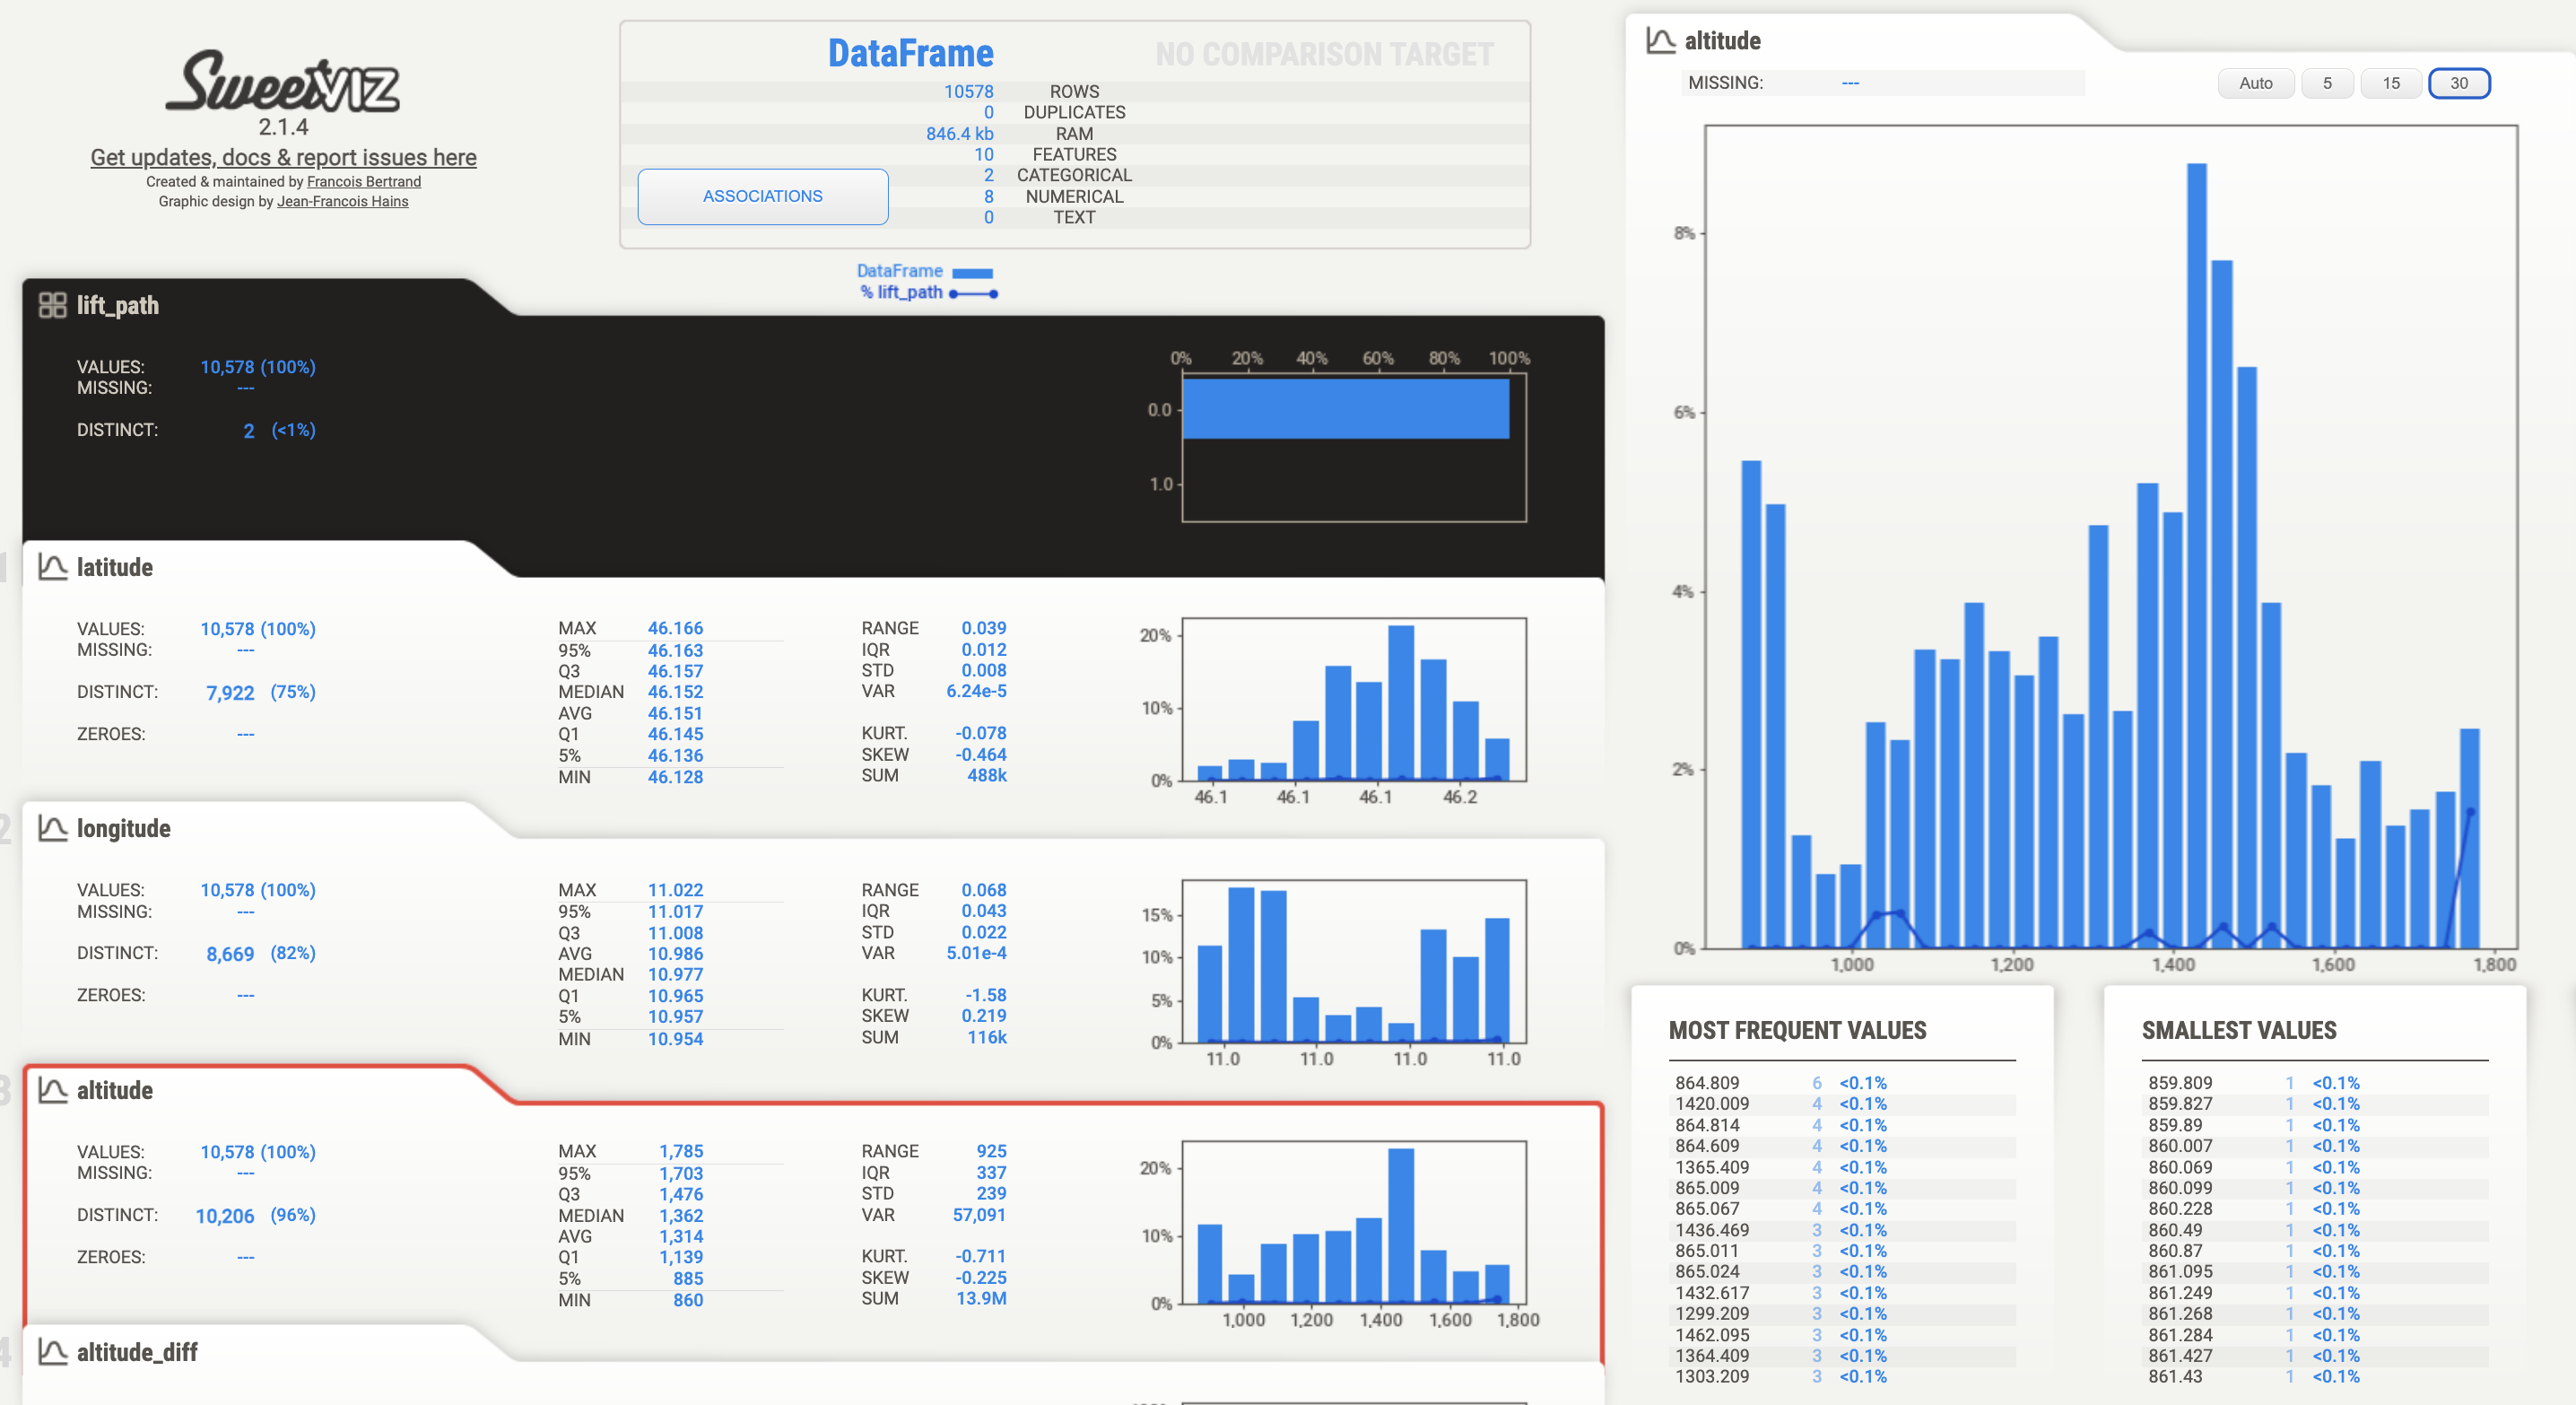
\includegraphics[width=\textwidth]{resources/data-report.png}
	\caption{Data visualization: \textit{(a)} left hand side, all the columns description, \textit{(b)} right hand side, altitude figure and the lift path bar chart}
	\label{fig:data-report}
\end{figure}

\subsection{Data correlation}
Additionally, within the scope of this study, an accurate evaluation of data correlation will be conducted. It refers to the relationship between two or more variables, describing how changes in one variable may correspond to changes in another. Correlation analysis helps uncover patterns and dependencies in data.



\begin{figure}[htb]
	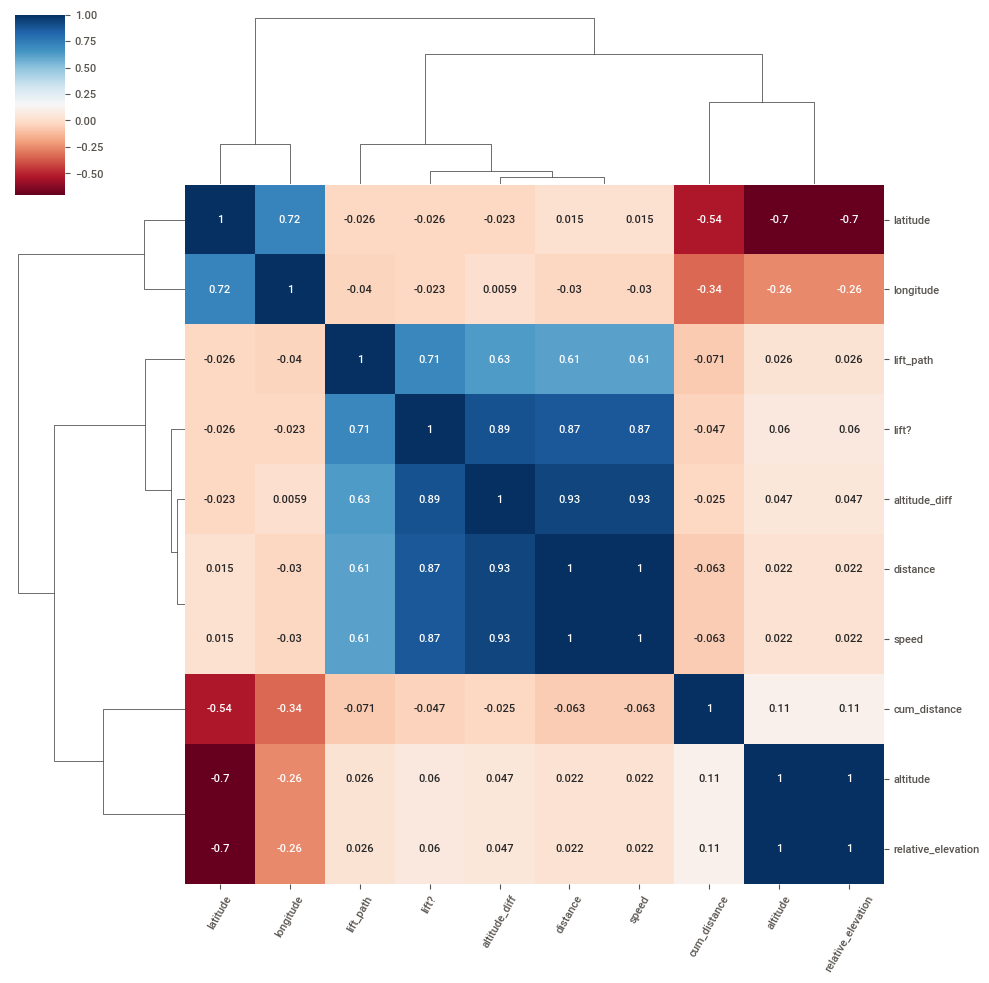
\includegraphics[width=\textwidth]{resources/correlation.png}
	\caption{Data correlation}
	\label{fig:correlation}
\end{figure}

Based on the provided illustration in  \ref*{fig:correlation}, it is evident that there exists a direct relationship or positive correlation between the lift variable and altitude difference, distance, as well as speed. This suggests that as there is a lift, there is a corresponding increase in altitude difference, distance, and speed. Unarguably, it's pretty evident that any mode of transportation will be faster than biking or skiing down.

\section{Conclusion}
\label{sec:data:conclusion}

To summarize, the main focus of this chapter was to process raw GPS data by loading it and transforming it into Pandas data frames. The data is then used for several calculations such as altitude, altitude difference, distance, cumulative distance, speed, lift detection, and lift path identification. The chapter also includes visualizing all the columns of the data frames and analyzing and data correlation. Finally, the variables with high correlation are selected as features to train ML models in
\textbf{Chapter \ref{sec:model}}

